\documentclass[aspectratio=169]{beamer}

% because we need to claim weird things
\newtheorem{claim}{Claim}
\newtheorem{defn}{Definition}
%\newtheorem{lemma}{Lemma}
\newtheorem{thm}{Theorem}
\newtheorem{vita}{Vit\ae}
\newtheorem{qotd}{Quote of the Day}

\usepackage{algorithm}
\usepackage{algpseudocode}
\usepackage{listings}
\usepackage{color}
\usepackage{graphics}
\usepackage{ulem}
\bibliographystyle{unsrt}

% background image
\usebackgroundtemplate%
{%
    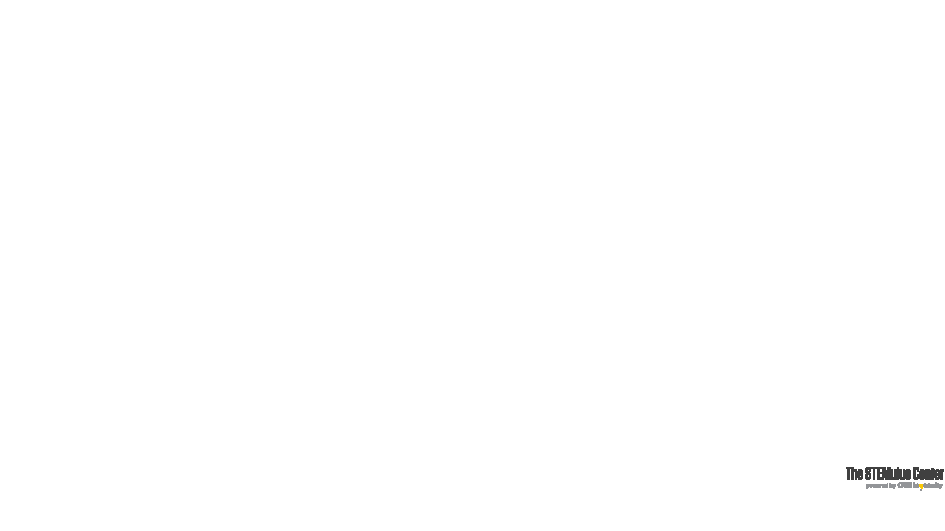
\includegraphics[width=\paperwidth,height=\paperheight]{../artifacts/stemulus.pdf}%
}
\setbeamertemplate{caption}[numbered]
\lstset{%
	breaklines=true,
	captionpos=b,
	frame=single,
	keepspaces=true,
	showstringspaces=false
}

% page numbers
\addtobeamertemplate{navigation symbols}{}{%
    \usebeamerfont{footline}%
    \usebeamercolor[fg]{footline}%
    \hspace{1em}%
    \insertframenumber/\inserttotalframenumber
}

% presentation header
\usetheme{Warsaw}
\title{Model-View-Controller}
\author{Dylan Lane McDonald}
\institute{CNM STEMulus Center\\Web Development with PHP}
\date{\today}

\begin{document}
\lstset{language=Java}
\begin{frame}
\titlepage
\end{frame}

\begin{frame}
\frametitle{Outline}
\tableofcontents
\end{frame}

\section{Design Patterns}
\begin{frame}
\frametitle{Design Patterns}
\begin{defn}
A \textbf{design pattern} is a reusable and accepted solution to a particular software engineering problem. Design patterns are not directly translatable into code. Instead, they provide a template that can be followed while implementing a particular solution.
\end{defn}
\pause
\mbox{}\\
That is, a design pattern can be thought more as a roadmap to a particular solution. Design patterns are a core principle of modern object oriented design and widely used and recognized in both academia and industry.

\mbox{}\\
There are several books on design patterns that form the foundation of today's web frameworks. \cite{codeComplete, designPatterns, j2ee}
\end{frame}

\begin{frame}
\frametitle{Commonly Used Design Patterns}
Many design patterns will be encountered in this class:
\begin{itemize}
	\item \textbf{Data Access Object:} Core design pattern for all mySQL-enabled classes
	\item \textbf{Iterator:} Provide a way to access elements one at a time
	\item \textbf{Observer:} An object, maintains a list of its observers, and notifies them automatically of any state changes, usually by calling one of their methods
	\item \textbf{Lazy Initialization:} Loading an object from a database on demand
	\item \textbf{Model-View-Controller:} Divides software into three interconnected parts, so as to separate how data is manipulated and presented to the user
\end{itemize}
The most important of which is \textbf{Model-View-Controller}, which is covered in more detail in the next slides.
\end{frame}

\section{Model-View-Controller}
\begin{frame}
\frametitle{Model-View-Controller}
\begin{defn}
\textbf{Model-View-Controller} is a design pattern for user interfaces. It clearly delineates the front and back end of a software solution by putting the front end in the view and the back end in the model \& controller.
\end{defn}
\pause
\mbox{}\\
Model-View-Controller's main advantage is to separate the frontend (View) component from the backend (Model) component and have the two meet in the middle (Controller) component. Following this design pattern will give rise to cleaner and better organized code.
\end{frame}

\begin{frame}
\frametitle{Model-View-Controller}
The three components of Model-View-Controller:
\begin{enumerate}
	\item \textbf{Model}: the data being represented. This is typically implemented as an object representing a database row.
	\item \textbf{View}: the screen the user sees. This usually is  HTML output of the model. 
	\item \textbf{Contoller}: the mechanism that allows for the manipulation of the model. This is usually input form that allows the user to modify or add to the model.
\end{enumerate}
Model-View-Controller is a commonly deployed design pattern in web programming. In fact, is is the entire basis for many web frameworks such as:
\begin{itemize}
	\item Java Enterprise Edition
	\item Laravel
	\item Ruby on Rails
\end{itemize}
\dots and many more
\end{frame}

\begin{frame}
\frametitle{Model-View-Controller}
\begin{figure}
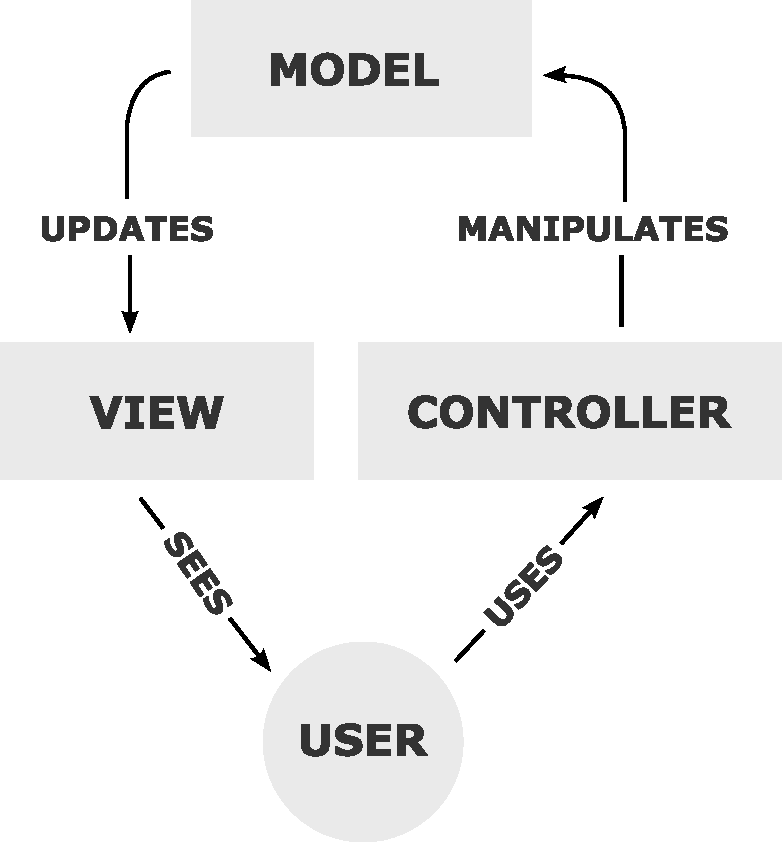
\includegraphics[scale=0.42]{../artifacts/mvc-diagram.pdf}
\caption{Model-View-Controller}
\label{fig:mvc}
\end{figure}
\end{frame}

\begin{frame}
\frametitle{Further Reading on Design Patterns}
\bibliography{mvc}
\end{frame}
\end{document}